\section{Interface 1}

On considère le problème à l'interface 1 uniquement (voir figure~\ref{iface1}).

\begin{figure}[!h]
    \centering{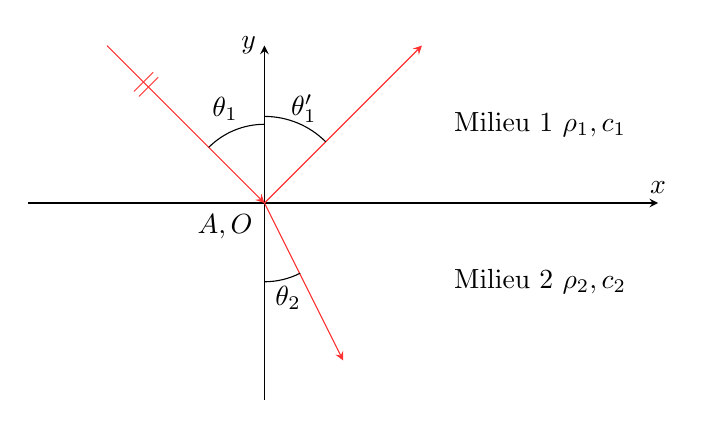
\begin{tikzpicture}

    % ifaces
    \draw [>=stealth, ->] (-3,0) -- (5,0);

    % Labels
    \draw (3.5,1) node {Milieu 1 $\rho_1,c_1$};
    \draw (3.5,-1) node {Milieu 2 $\rho_2,c_2$};

    % verticals
    \draw [dashed] (0,1.5) -- (0,-1.5);

    % axis
    %% y
    \draw [>=stealth, ->] (0,-2.5) -- (0,2);
    \draw (-.2,2) node {$y$};
    %% x (already drawn)
    \draw (5,.2) node {$x$};


    % points A & B
    \draw (-.5, -.3) node {$A,O$};

    % rays
    \draw [red!80, >=stealth, ->] (-2,2) -- (0,0) node[near start, sloped] {$| |$};
    \draw [red!80, >=stealth, ->] (0,0) -- (2,2);
    \draw [red!80, >=stealth, ->] (0,0) -- (1, -2);

    % angles
    \draw (0,1) arc (90:135:1) node at (-0.5,1.2) {$\theta_1$};
    \draw (0,1.1) arc (90:45:1.1) node at (0.5,1.2) {$\theta_1'$};
    \draw (0,-1) arc (-90:-63:1) node at (0.3,-1.2) {$\theta_2$};

\end{tikzpicture}
}
    \caption{\label{iface1} Considération des effets à l'interface 1}
\end{figure}

\subsection{Position du problème}


\paragraph{Pressions totales} Dans le milieu 1, la pression totale vérifie :

\begin{equation}
    \left(\Delta - \frac{1}{c_1^2}\frac{\partial^2}{\partial t^2}\right)\pTOT_1(x,y,t) = 0 \;;\; \forall x,t \,\mathrm{et}\, \forall y \geq 0 \label{i1_prop1}
\end{equation}


Dans le milieu 2, la pression totale vérifie :

\begin{equation}
    \left(\Delta - \frac{1}{c_2^2}\frac{\partial^2}{\partial t^2}\right)\pTOT_2(x,y,t) = 0 \;;\; \forall x,t\,\mathrm{et}\,\forall y \leq 0 \label{i1_prop2}
\end{equation}


\paragraph{Champ monochromatique} Les ondes sont considérées monochromatiques, l'équation d'Helmholtz est donc vérifiée
dans chacun des milieux :

\begin{eqnarray}
    (\Delta + k_1^2)p_1(x,y) & = & 0 \;;\; \forall x,t \label{i1_helm1}\\
    (\Delta + k_2^2)p_2(x,y) & = & 0 \;;\; \forall x,t \label{i1_helm2}
\end{eqnarray}

On définit les nombres d'onde $k_i = \nicefrac{\omega_i}{c_i}$, $\omega_i$ étant la pulsation de l'onde dans le milieu
$i$ ($i\in \{1,2\}$).

\paragraph{Condition de Sommerfeld}

\paragraph{Conditions à l'interface}

A l'interface, il y a continuité des pressions et des vitesses normales. Ainsi :

\begin{eqnarray}
    \pTOT_1(x, y=0, t) &=& \pTOT_2(x,y=0,t) \;;\;\forall x,t \label{i1_cl1}\\
    \vTOT_1(x, y=0, t) &=& \vTOT_2(x,y=0,t) \;;\;\forall x,t \label{i1_cl2}
\end{eqnarray}

Dans le milieu 2, on ne considérera que l'onde transmise, ainsi pour les equations~\eqref{i1_prop2},~\eqref{i1_cl1}
et~\eqref{i1_cl2}, on aura :

\begin{eqnarray*}
    \pTOT_2 = \pT_1\\
    \vTOT_2 = \vT_1
\end{eqnarray*}

On définit alors :

$$\pTOT_1 = \pI_1 + \pR_1$$

\subsection{Forme générale des pressions}

Les ondes sont considérés monochromatiques :

\begin{eqnarray}
    \pI_1(x,y,t) & = & A_1e^{j(\omega_1t-k_1\sin\theta_1x+k_1\cos\theta_1y)} \label{i1_pgeni}\\
    \pR_1(x,y,t) & = & B_1e^{j(\omega_1t-k_1\sin\theta_1'x+k_1\cos\theta_1'y)} \label{i1_pgenr}\\
    \pT_1(x,y,t) & = & A_2e^{j(\omega_2t-k_2\sin\theta_2x+k_2\cos\theta_2y)} \label{i1_pgent}
\end{eqnarray}

\subsection{Forme générales des vitesses normales}

On sait que les vitesses normales ont une expression de la forme : $v_i(x,y,t) = v_i(x,y)e^{j\omega_it}$, d'après
l'équation d'Euler, on peut écrire :

\begin{eqnarray}
    \rho_1\frac{\partial\vTOT_1}{\partial t} = -\frac{\partial\pTOT_1}{\partial y}
        & \Leftrightarrow & \vTOT_1 = -\frac{1}{j\omega_1\rho_1}\frac{\partial\pTOT_1}{\partial y}\label{i1_euler1}\\
    \rho_2\frac{\partial\vT_1}{\partial t} = -\frac{\partial\pT_1}{\partial y}
        & \Leftrightarrow & \vT_1 = -\frac{1}{j\omega_2\rho_2}\frac{\partial\pT_1}{\partial y}\label{i1_euler2}
\end{eqnarray}

\subsubsection{Calcul de $\vTOT_1$}


